\chapter{La gestion de version} % (fold)
\label{cha:La gestion de version}

\begin{it}
J'ai eu pour objectif de déployer un nouvel outil de gestion de version
dans l'entreprise. Cette partie évoque les détails de cette mise en
\oe{}uvre. Pour l'anecdote Git fut choisi comme remplacement à
Subversion lorsque \bsc{M.~Dubourg} consulta mon curiculum-vitae.
\end{it}

\section{Git : Le gestionnaire de code source} % (fold)%{{{
\label{sec:Git : Le gestionnaire de code source}

\lettrine{L}{es} logiciels de gestion de versions ou VCS\,
\footnote{\emph{Version Control System.}} sont utilisés principalement
par les développeurs. En effet, ils sont quasi exclusivement utilisés
pour gérer des codes sources, car ils sont capables de suivre
l’évolution d’un fichier texte \emph{ligne de code par ligne de code.}
Ces logiciels sont fortement conseillés pour gérer un projet
informatique.

Ceux-ci retiennent qui a effectué chaque modification de chaque fichier
et pourquoi. Ils sont par conséquent capables de dire qui a écrit chaque
ligne de chaque fichier et dans quel but ; si deux personnes travaillent
simultanément sur un même fichier, ils sont capables de fusionner leurs
modifications et d’éviter que le travail d’une de ces personnes ne soit
écrasé. La figure~\ref{flow} qui ce trouve en page \pageref{flow}
illustre basiquement l'utilisation de Git.

Ces logiciels ont donc par conséquent deux utilités principales :
\begin{itemize}

  \item suivre l’évolution d’un code source, pour retenir les
    modifications effectuées sur chaque fichier et être ainsi capable de
    revenir en arrière en cas de problème ;

  \item travailler à plusieurs, sans risquer de se marcher sur les
    pieds.  Si deux personnes modifient un même fichier en même temps,
    leurs modifications doivent pouvoir être fusionnées sans perte
    d’information.

\end{itemize}

\begin{figure}
  \begin{center}
    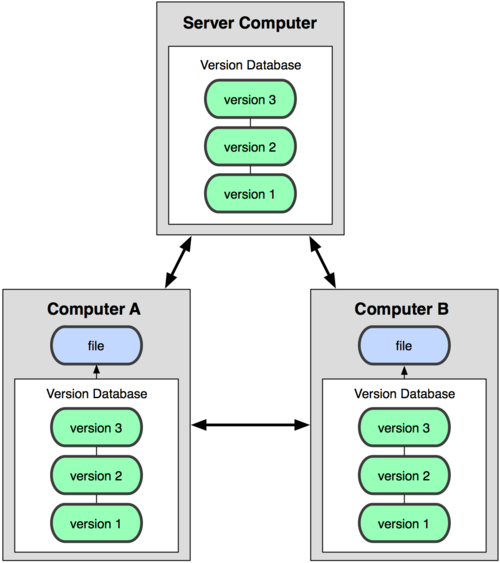
\includegraphics[scale=1.57]{images/workflow.png}
    \caption{ Chaque utilisateur possède une copie du code source
    ainsi que toutes les versions précédentes de celui-ci, ce qui n'est pas
    le cas de l'existant. Le serveur sert de point de rencontre entre les
    développeurs et possède lui aussi l’historique des versions.}
    \label{flow}
  \end{center}
\end{figure}

\subsection{L'installation} % (fold)%{{{
\label{sub:L'installation}

À peu près au milieu du stage, nous nous sommes heurtés à un problème
technique. Le serveur de l'entreprise ne contenait pas de version
récente de Git. En sachant que celui-ci est de type mutualisé\,
\footnote{C'est un concept d'hébergement dont la caractéristique
principale est d'être partagé par plusieurs utilisateurs.}, nous
n'avions pas les autorisations nécessaires pour installer une nouvelle
version.

Les logiciels libres sont réputés pour être rétro-compatibles, mais en
toute logique ils ne disposent pas des nouveautés sans les mettre à jour.
Le problème est qu'on ne pouvait pas créer des branches distantes dites
\og de suivi \fg{}. Cette fonctionnalité permet à plusieurs développeurs
de travailler en même temps sur une branche différente de celle par
défaut, par exemple pour expérimenter de nouvelles implémentations à
plusieurs.

À ce moment-là j'ai été très déçu et pensais mon travail inutilisable.
Cependant, mes efforts n'ont pas été vains puisque \bsc{M.~Dubourg} après
quelques recherches, a trouvé sur internet un utilisateur ayant réussi à
installer Git sur un serveur mutualisé.  Nous n'avions pas les droits
d'accès aux dossiers des programmes mais rien ne nous empêchait de
compiler Git à partir des sources pour nous permettre de créer en local
le logiciel\, \footnote{Le problème ne se serait pas posé si j'avais lu
le chapitre traitant de la compilation dans mon livre Linux, je n'ai
découvert cette méthode qu'après le stage\dots}. Ceci étant fait, en
redéfinissant la variable système qui stocke les chemins des
applications, nous avons pu utiliser notre compilé dernier cri.
% subsection L'installation (end)%}}}
% section Git : Le gestionnaire de code source (end)%}}}

\section{Le tutoriel utilisateur} % (fold)%{{{
\label{sec:Le tutoriel utilisateur}

Pour aider les développeurs à intégrer le nouveau gestionnaire de
version, j'ai élaboré un document Office Word de
quatorze pages qui explique les bases du logiciel, la mise en place de
l'outil dans leur environnement de travail respectif et l'utilisation de
celui-ci avec le gratuiciel TortoiseGit.  Pour être au plus près des
problématiques qui pourraient être rencontrées, j'ai conçu l'intégralité
du guide sous forme de questions et de réponses.

\begin{enumerate}
  \item Les bases
  \item Comment mettre en place Git sur Windows ?
  \item Comment gérer les dépôts Git ?
  \item Comment utiliser Git ?
  \item Comment utiliser les branches ?
  \item Comment consulter l'historique des modifications ?
  \item Quelle est la méthode de travail ?
\end{enumerate}
% section Le tutoriel utilisateur (end)%}}}

\section{Les utilitaires} % (fold)%{{{
\label{sec:Les utilitaires}

Nous avons longuement discuté sur le côté technique de Git. En effet cet
outil est à la base un logiciel libre provenant de Linux et n'a pas
d'interface graphique, ce choix est établi sur le fait qu'un développeur
n'a pas forcément besoin de cela pour travailler\, \footnote{Sans nul
doute que pour un graphiste, une souris est un élément indispensable
pour ses créations, mais pas pour produire du code.} et aussi que ce
logiciel regorge de fonctionnalités et donc très difficile à simplifier
à travers une interface ne pouvant fonctionner qu'avec une souris.
L'équipe n'étant pas très férue de ligne de commande et le logiciel
TortoiseGit ne reprenant que les fonctions essentielles de Git, il a
fallu que je conçois des petits programmes qui fonctionnent en un clic
pour simplifier les choses répétitives.

\subsection{Lister les dépôts du serveur} % (fold)%{{{
\label{sub:Lister les dépôts du serveur}

Mon travail suivant consista à lister les dépôts Git sur une page Web.
Le serveur OVH centralise les codes sources de la société, les
développeurs, eux doivent récupérer une copie des dossiers pour pouvoir
travailler dessus. Seulement, lancer FilleZilla\, \footnote{FileZilla
est un logiciel gratuit qui permet de se connecter à distance sur un
serveur pour y télécharger des fichiers via le Protocole FTP.} pour
connaître les noms des répertoires Git puis recopier le bon lien
hypertexte avec le bon chemin d'arborescence est une tâche fastidieuse.
J'ai donc, à l'aide de mes connaissances en système UNIX, créé un script
qui analyse un dossier défini et qui liste les différents dépôts tout en
leur mettant les bonnes adresses de téléchargement en préfixe comme nous
le montre la figure~\ref{repo} en page \pageref{repo}. Du coup, un
simple copier-coller du lien du dépôt voulu dans tortoiseGit suffit pour
cloner, gain de productivité et de simplicité réunies.

\begin{figure}
    \begin{center}
        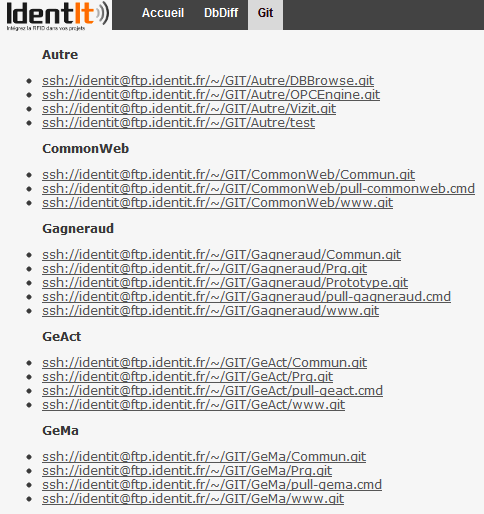
\includegraphics[scale=0.8]{images/repo.png}
        \caption{La liste des dépôts cliquables.}
        \label{repo}
    \end{center}
\end{figure}

\newpage
% subsection Lister les dépôts du serveur (end)%}}}

\subsection{Mise en production automatique} % (fold)%{{{
\label{sub:Mise en production automatique}

Une fois que les développeurs sont satisfaits de leurs modifications,
ils doivent mettre à jour le dépôt distant pour partager leurs travaux.
Une fois les modifications validées par le chef de projet, celui-ci doit
mettre en ligne sur le dépôt de production. J'ai créé un script Batch\,
\footnote{Désigne un fichier qui contient une suite de commandes qui
seront traitées automatiquement par Windows.} \og modèle \fg{} pour
que cela se fasse en un clic.
% section Mise en production automatique (end)%}}}

\subsection{Mise à jour locale automatique} % (fold)%{{{
\label{sub:Mise à jour locale automatique}

Les développeurs possèdent des clones des dépôts distants en local pour
bien évidemment maintenir le code source. Le fait qu'il y ait une
multitude de dépôts implique une mise à jour des clones locaux pour
récupérer les modifications des autres développeurs ce qui est très
répétitif. J'ai donc créé un script Batch qui explore tous les dossiers
englobant les sources des dépôts et les met à jour. Pour cela j'ai
parcouru la documentation de la console Windows et ça n'a pas été
évident du tout. Pour l'anecdote, je devais à partir de mon MacBook
Pro\, \footnote{Mac OS X est un système de type UNIX.} ; lancer une
machine virtuelle Windows\, \footnote{À partir du logiciel VirtualBox.}
; pour créer mon script qui s'exécute en console ; et qui lance enfin un
terminal Linux pour faire la mise à jour\dots
% subsection Mise à jour locale automatique (end)%}}} section Les
% utilitaires (end)%}}}
